\documentclass[fontsize=10pt,a4paper]{scrartcl}

\usepackage{../../styles/myusepackages}
\usepackage{../../styles/mypythonstyle}
\usepackage{../../styles/myMCquestions}
\usepackage{../../styles/myframedenv}
%If graphics is listed before,some problems arise
\usepackage{graphicx}

\usepackage[english]{babel}
\usepackage[english,verbose]{layout}
\hypersetup{pdflang={es-ES}}

\newcommand{\academicyear}{2023-2024}
%%%%%%%%%%%%%%%%%%%%%%%%%%%%%%%%%%%%%%%%%%%%%%%%
%%%%%%%%%%%% TITLE
\title{Programming in Python\\ TEMA 8}
\usepackage{etoolbox}
\makeatletter
\providecommand{\subtitle}[1]{% add subtitle to \maketitle
  \apptocmd{\@title}{\par {\Huge #1 \par}}{}{}
}
\makeatother
\subtitle{\Large{Mutabilidad}}
\author{Universidad Politécnica de Valencia}
\date{\academicyear{}}
%%%%%%%%%%%%%%%%%%%END TITLE%%%%%%%%%%%%%%%%%%%%%

\begin{document}
\maketitle
\tableofcontents


\chapter*{Prólogo}
\addcontentsline{toc}{chapter}{Prólogo}


¡Bienvenido a este libro de Python que te acompañará en el tema de programación durante el primer semestre de tus estudios universitarios!

Este libro se inspira en dos obras de código abierto:\textit{Python for Everybody} de Charles Severance \cite{severance2016python} y \textit{Think Python: How to Think Like a Computer Scientist} de Allen Downey \cite{downey2016thinkpython}. Estos libros han compartido su conocimiento bajo licencias de Creative Commons, formando la base del contenido de este libro.

La motivación para crear este libro surge de la necesidad de comprender sólidamente las pruebas (o el «testing») en la educación de programación. Creemos que las pruebas son una habilidad esencial en el mundo de la programación, pero sorprendentemente, este aspecto crucial a menudo se pasa por alto en los libros de programación para principiantes. Con el libro que tienes en tus manos, buscamos cambiar eso.

Integrar el «testing» en un curso de programación para principiantes no es fácil. Es por eso que utilizamos el innovador enfoque TILE \cite{10132188} «Test Informed Learning with Examples» o el Aprendizaje Informado por Pruebas con Ejemplos. El enfoque TILE se centra en integrar las pruebas de software en tu experiencia de programación introductoria de manera efectiva y placentera. TILE fue desarrollado con el generoso apoyo y financiamiento del proyecto Erasmus+ QPeD (número de contrato 2020-1-NL01-KA203-064626) y del proyecto ENACTEST (número de proyecto 101055874).

Con TILE, las pruebas se convierten en una parte integral de tu trayecto de programación desde el principio. Creemos firmemente que las pruebas no deben ser una idea secundaria, sino un aspecto esencial de tu proceso de codificación. Por eso te presentamos las pruebas desde el primer programa de ejemplo que encuentres.

Nuestro objetivo es dotarte del conocimiento y las habilidades para que te conviertas en un programador Python competente, armado con el poder de las pruebas para crear programas de alta calidad.

Así que, mientras te sumerges en el emocionante mundo de Python, recuerda que este libro está aquí para guiarte paso a paso en el dominio tanto de la programación como de las pruebas. Juntos, embarquémonos en este viaje mientras exploramos las maravillas de Python y el arte de las pruebas de software.

¡Feliz aprendizaje!

Tanja Vos
(tvos@dsic.upv.es)

%!TEX root=main_tema7.tex

\section{Las listas son mutables}
\label{mutable}
\index{lista!elemento}
\index{acceso}
\index{indice@índice}
\index{operador!de corchetes}
\index{corchetes!operador de}

La sintaxis para acceder a los elementos de una lista es la misma que para
acceder a los caracteres de una cadena: el operador de corchetes.  La
expresión dentro de los corchetes especifica el índice.  Recuerda que los
índices comienzan en 0:

\begin{Verbatim}[frame=single]
>>> quesos = ['Cheddar', 'Edam', 'Gouda']
>>> quesos[0]
'Cheddar'
\end{Verbatim}
%
A diferencia de las cadenas, las listas son mutables.  Cuando el operador de corchetes aparece
en el lado izquierdo de una asignación, este identifica el elemento de la
lista que será asignado.
\index{mutabilidad}

\begin{Verbatim}[frame=single]
>>> numeros = [42, 123]
>>> numeros[1] = 5
>>> numeros
[42, 5]
\end{Verbatim}
%
El uno-ésimo elemento de \texttt{numeros}, que
solía ser 123, ahora es 5.
%
La Figura~\ref{fig.liststate} muestra
el diagrama de estado para \texttt{quesos}, \texttt{numeros} y \texttt{vacio}.
\index{diagrama!de estado}
\index{estado, diagrama de}

\begin{figure}
\centerline
{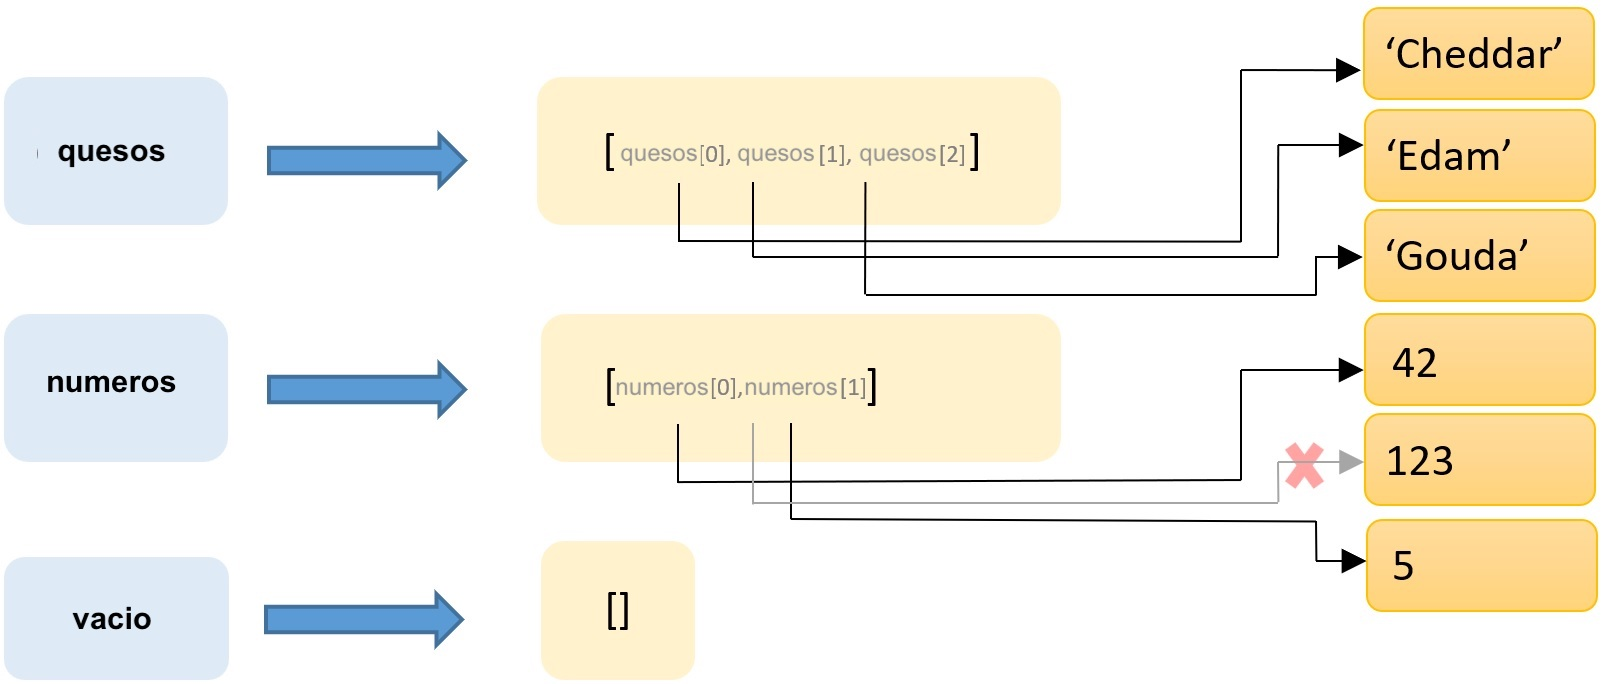
\includegraphics[scale=0.3]{images/state-diagram.jpg}}
\caption{Diagrama de estado.}
\label{fig.liststate}
\end{figure}

Las listas se representan por cajas con la palabra ``list'' por fuera
y los elementos de la lista por dentro.  \texttt{quesos} se refiere a
una lista con tres elementos con índices 0, 1 y 2.
\texttt{numeros} contiene dos elementos; el diagrama muestra que el
valor del segundo elemento ha sido reasignado de 123 a 5.
\texttt{vacio} se refiere a una lista sin elementos.
\index{asignación de ítem}
\index{item@ítem!asignación de}
\index{reasignación}


\section{Métodos de lista}
\index{lista!método de}
\index{metodo@método!de lista}

Python proporciona métodos que operan en listas.  
Métodos se llaman con la notación del punto, como veremos en el ejemplo abajo
\pythoninline{t.append('d')}.
Por ejemplo,
\texttt{append} agrega un nuevo elemento al final de la lista:
\index{metodo@método!append}
\index{append, método}

\begin{Verbatim}[frame=single]
>>> t = ['a', 'b', 'c']
>>> t.append('d')
>>> t
['a', 'b', 'c', 'd']
\end{Verbatim}



\texttt{extend} toma otra lista como argumento y anexa todos
los elementos:
\index{metodo@método!extend}
\index{extend, método}

\begin{Verbatim}[frame=single]
>>> t1 = ['a', 'b', 'c']
>>> t2 = ['d', 'e']
>>> t1.extend(t2)
>>> t1
['a', 'b', 'c', 'd', 'e']
\end{Verbatim}
%
Este ejemplo deja a \texttt{t2} sin modificar.

\texttt{sort} ordena los elementos de la lista de menor a mayor:
\index{metodo@método!sort}
\index{sort, método}

\begin{Verbatim}[frame=single]
>>> t = ['d', 'c', 'e', 'b', 'a']
>>> t.sort()
>>> t
['a', 'b', 'c', 'd', 'e']
\end{Verbatim}
%
La mayoría de los métodos de lista son nulos: modifican la lista y devuelven \texttt{None}.
Si por casualidad escribes \texttt{t = t.sort()}, te decepcionará
el resultado.
\index{metodo@método!nulo}
\index{nulo, método}
\index{valor especial!None}
\index{None, valor especial}




\section{Eliminar elementos}
\index{eliminación de elementos}
\index{elemento!eliminación}

Hay varias maneras de eliminar elementos de una lista.  Si conoces
el índice del elemento que quieres, puedes utilizar el método
\pythoninline{pop}:
\index{metodo@método!pop}
\index{pop, método}

\begin{Verbatim}[frame=single]
>>> t = ['a', 'b', 'c']
>>> x = t.pop(1)
>>> t
['a', 'c']
>>> x
'b'
\end{Verbatim}
%
\pythoninline{pop} modifica la lista y devuelve el elemento que se eliminó.
Si no entregas un índice, elimina y devuelve el
último elemento.

Si no necesitas el valor eliminado, puedes utilizar el
operador \pythoninline{del}:
\index{operador!del}
\index{del, operador}

\begin{Verbatim}[frame=single]
>>> t = ['a', 'b', 'c']
>>> del t[1]
>>> t
['a', 'c']
\end{Verbatim}
%
Si conoces el elemento que quieres eliminar (pero no el índice),
puedes utilizar el método \pythoninline{remove}:
\index{metodo@método!remove}
\index{remove, método}

\begin{Verbatim}[frame=single]
>>> t = ['a', 'b', 'c']
>>> t.remove('b')
>>> t
['a', 'c']
\end{Verbatim}
%
El valor de retorno de \pythoninline{remove} es \pythoninline{None}.
\index{valor especial!None}
\index{None, valor especial}

Para eliminar más de un elemento, puedes utilizar \pythoninline{del} con
índices de trozo o corte:

\begin{Verbatim}[frame=single]
>>> t = ['a', 'b', 'c', 'd', 'e', 'f']
>>> del t[1:5]
>>> t
['a', 'f']
\end{Verbatim}
%
Como siempre, el trozo selecciona todos los elementos hasta el segundo índice
pero sin incluirlo.



\section{Listas y cadenas}
\index{lista}
\index{cadena}
\index{secuencia}

Una cadena es una secuencia de caracteres y una lista es una secuencia
de valores, pero una lista de caracteres no es lo mismo que una
cadena.  Para convertir una cadena en una lista de caracteres,
puedes utilizar la función \pythoninline{list}:
\index{list, función}
\index{función!list}

\begin{Verbatim}[frame=single]
>>> s = 'spam'
>>> t = list(s)
>>> t
['s', 'p', 'a', 'm']
\end{Verbatim}
%
Dado que \pythoninline{list} es el nombre de una función predefinida, deberías
evitar utilizarlo como nombre de variable.  Además es buena practica evitar la letra \pythoninline{l} porque se parece mucho al numero \pythoninline{1}.  Entonces por eso usamos aqui \pythoninline{t}.

La función \pythoninline{list} separa la cadena en letras individuales.  Si
quieres separar una cadena en palabras, puedes utilizar
el método \pythoninline{split}:
\index{metodo@método!split}
\index{split, método}

\begin{Verbatim}[frame=single]
>>> s = 'pining for the fjords'
>>> t = s.split()
>>> t
['pining', 'for', 'the', 'fjords']
\end{Verbatim}
%
Un argumento opcional llamado \textbf{ delimitador} especifica qué
caracteres usar como separador de palabras.
El siguiente ejemplo
usa un guión como delimitador:
\index{argumento opcional}
\index{opcional!argumento}
\index{delimitador}

\begin{Verbatim}[frame=single]
>>> s = 'spam-spam-spam'
>>> delimitador = '-'
>>> t = s.split(delimitador)
>>> t
['spam', 'spam', 'spam']
\end{Verbatim}
%
\pythoninline{join} es el inverso de \pythoninline{split}.
Toma una lista de cadenas y
concatena los elementos.  \pythoninline{join} es un método de cadena,
por lo que tienes que invocarlo en el delimitador y pasarle la
lista como parámetro:
\index{metodo@método!join}
\index{join, método}
\index{concatenación}

\begin{Verbatim}[frame=single]
>>> t = ['pining', 'for', 'the', 'fjords']
>>> delimitador = ' '
>>> s = delimitador.join(t)
>>> s
'pining for the fjords'
\end{Verbatim}
%
En este caso el delimitador es un carácter de espacio, por lo que
\pythoninline{join} pone un espacio entre las palabras.  Para concatenar
cadenas sin espacios, puedes usar la cadena vacía,
\verb"''", como delimitador.
\index{cadena!vacía}
\index{vacía!cadena}


\section{Objetos, valores e igualdad}
\label{equivalence}
\index{objeto}
\index{valor}

Si ejecutamos estas sentencias de asignación:

\begin{python}[frame=single]
a = 'banana'
b = 'banana'
\end{python}
%
sabemos que las variables \pythoninline{a} y \pythoninline{b} se refieren a una
cadena, pero no sabemos si se refieren a la {\em misma} cadena.
Hay dos estados posibles, mostrados en la Figura~\ref{fig.list1}.
\index{alias}

\begin{figure}
\centerline
{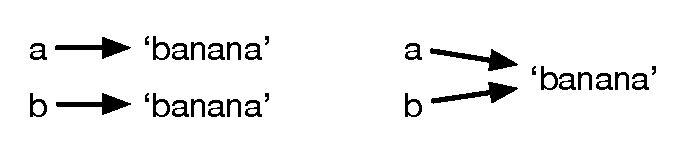
\includegraphics[scale=0.8]{images/list1.eps}}
\caption{Variables y sus referencias a valores}
\label{fig.list1}
\end{figure}

En el primer caso, \texttt{a} y \texttt{b} se refieren a dos objetos diferentes que
tienen el mismo valor.  En el segundo caso, se refieren al mismo
objeto.
\index{operador!is}
\index{is, operador}

Para verificar si dos variables se refieren al mismo objeto, puedes
usar el operador \pythoninline{is}.

\begin{Verbatim}[frame=single]
>>> a = 'banana'
>>> b = 'banana'
>>> a is b
True
>>> a == b
True
\end{Verbatim}
%
En este ejemplo, Python solo crea un objeto de cadena y tanto \pythoninline{a} como \pythoninline{b} se refieren a este.  Pero cuando creas dos listas, Python lo hace diferente y nos da
dos objetos:

\begin{Verbatim}[frame=single]
>>> a = [1, 2, 3]
>>> b = [1, 2, 3]
>>> a is b
False
>>> a == b 
True
\end{Verbatim}
%


En este caso diríamos que las dos listas son \textbf{equivalentes},
porque tienen los mismos elementos, pero no \textbf{idénticos}, porque
no son el mismo objeto.  Si dos objetos son idénticos, son
también equivalentes, pero si son equivalentes, no necesariamente son
idénticos.
\index{equivalencia}
\index{identidad}

Hasta ahora, hemos estado utilizando ``objeto'' y ``valor''
indistintamente, pero es más preciso decir que un objeto tiene un
valor.  Si evalúas \pythoninline{[1, 2, 3]}, obtienes un objeto de
lista cuyo valor es una secuencia de enteros.  Si otra
lista tiene los mismos elementos, decimos que tiene el mismo valor, pero
no es el mismo objeto.
\index{objeto}
\index{valor}


\section{Alias}
\index{alias}
\index{referencia!alias}

Si \texttt{a} se refiere a un objeto y asignas \texttt{b = a},
entonces ambas variables se refieren al mismo objeto:

\begin{Verbatim}[frame=single]
>>> a = [1, 2, 3]
>>> b = a
>>> b is a
True
\end{Verbatim}
%

La asociación de una variable con un objeto se llama \textbf{
referencia}.  En este ejemplo, hay dos referencias al mismo
objeto.
\index{referencia}

Un objeto con más de una referencia tiene más
de un nombre, por lo que decimos que el objeto tiene un \textbf{ alias}.
\index{mutabilidad}

Si el objeto con alias es mutable, los cambios realizados con un alias afectan
al otro:

\begin{Verbatim}[frame=single]
>>> a = [1, 2, 3]
>>> b = a
>>> b[0] = 42
>>> a
[42, 2, 3]
\end{Verbatim}
%
Aunque este comportamiento puede ser útil, es propenso a errores.  En general,
es más seguro evitar los alias cuando trabajes con objetos
mutables.
\index{inmutabilidad}

Para los objetos inmutables como las cadenas, los alias no son tan
problemáticos.  En este ejemplo:

\begin{Verbatim}[frame=single]
a = 'banana'
b = 'banana'
\end{Verbatim}
%
casi nunca hace una diferencia si \texttt{a} y \texttt{b} se refieren
a la misma cadena o no.


\section{Argumentos de lista}
\label{list.arguments}
\index{lista!como argumento}
\index{argumento}
\index{argumento de lista}
\index{referencia}
\index{parámetro}

Cuando pasas una lista como argumento a una función, la función obtiene una referencia a
la lista.  Si la función modifica la lista, la sentencia llamadora ve
el cambio.  Por ejemplo, \pythoninline{sin_cabeza} quita el primer elemento
de una lista:

\begin{python}[frame=single]
def sin_cabeza(t):
    del t[0]
\end{python}
%
Se utiliza de la siguiente manera:

\begin{Verbatim}[frame=single]
>>> letras = ['a', 'b', 'c']
>>> sin_cabeza(letras)
>>> letras
['b', 'c']
\end{Verbatim}
%
El parámetro \pythoninline{t} y la variable \pythoninline{letras} son
alias para el mismo objeto.  

Es importante distinguir entre operaciones que
modifican listas y operaciones que crean nuevas listas.  Por
ejemplo, el método \texttt{append} modifica una lista, pero el
operador \texttt{+} crea una nueva lista.
\index{metodo@método!append}
\index{append, método}
\index{lista!concatenación}
\index{concatenación!lista}

Aquí hay un ejemplo que utiliza \texttt{append}:
%
\begin{Verbatim}[frame=single]
>>> t1 = [1, 2]
>>> t2 = t1.append(3)
>>> t1
[1, 2, 3]
>>> t2
None
\end{Verbatim}
%
El valor de retorno de \texttt{append} es \texttt{None}.

Aquí hay un ejemplo que utiliza el operador \texttt{+}:
%
\begin{Verbatim}[frame=single]
>>> t3 = t1 + [4]
>>> t1
[1, 2, 3]
>>> t3
[1, 2, 3, 4]
\end{Verbatim}
%
El resultado del operador es una lista nueva y la lista original no ha
cambiado.

Esta diferencia es importante cuando escribes funciones que
se supone que modifican listas.  Por ejemplo, esta función
{\em NO} elimina la cabeza de una lista:
%
\begin{python}[frame=single]
def sin_cabeza_mal(t):
    t = t[1:]              
\end{python}
%
El operador de trozo crea una nueva lista y la asignación
hace que \pythoninline{t} se refiera a esta, pero eso no afecta a la llamadora.
\index{operador!de trozo}\index{slice}
\index{trozo!operador}
%
\begin{Verbatim}[frame=single]
>>> t4 = [1, 2, 3]
>>> sin_cabeza_mal(t4)
>>> t4
[1, 2, 3]
\end{Verbatim}
%
Al principio de \pythoninline{sin_cabeza_mal}, \pythoninline{t} y \pythoninline{t4}
se refieren a la misma lista.  Al final, \pythoninline{t} se refiere a una nueva lista,
pero \pythoninline{t4} aún se refiere a la original, la lista sin modificar.

Una alternativa es escribir una función que cree y
devuelva una nueva lista.  Por
ejemplo, \pythoninline{cola} devuelve todos los elementos
de una lista excepto el primero:

\begin{python}[frame=single]
def cola(t):
    return t[1:]
\end{python}
%
Esta función deja a la lista original sin modificar.
Se utiliza de la siguiente manera:

\begin{Verbatim}[frame=single]
>>> letra = ['a', 'b', 'c']
>>> resto = cola(letras)
>>> resto
['b', 'c']
\end{Verbatim}



\section{Depuración}
\index{depuración}

El uso descuidado de las listas (y otros objetos mutables)
puede llevar a largas horas de depuración.  Aquí hay algunas
trampas comunes y maneras de evitarlas:

\begin{enumerate}

\item La mayoría de los métodos de lista modifican el argumento y
  devuelven \pythoninline{None}. Esto es lo opuesto a los métodos de cadena,
  que devuelven una nueva cadena y dejan sola a la original.

Si te acostumbraste a escribir código de cadena como este:

\begin{python}[frame=single]
palabra = palabra.strip()
\end{python}

Es tentador escribir código de lista como este:

\begin{python}[frame=single]
t = t.sort()           
\end{python}
\index{metodo@método!sort}
\index{sort, método}

Pero, dado que \pythoninline{sort} devuelve \pythoninline{None}, es probable que la
siguiente operación que realices con \pythoninline{t} falle.

Antes de utilizar métodos y operadores de lista, deberías leer la
documentación cuidadosamente y luego probarlos en modo interactivo.

\item Escoge una forma y quédate con esa.

Parte del problema con las listas es que hay muchas
maneras de hacer las cosas.  Por ejemplo, para eliminar un elemento de
una lista, puedes utilizar \pythoninline{pop}, \pythoninline{remove}, \pythoninline{del},
o incluso una asignación de trozo.

Para agregar un elemento, puedes utilizar el método \pythoninline{append} o
el pythoninline \texttt{+}.  Suponiendo que \pythoninline{t} es una lista y
\pythoninline{x} es un elemento de lista, estas líneas son correctas:

\begin{Verbatim}[frame=single]
t.append(x)
t = t + [x]
t += [x]
\end{Verbatim}

Y estas son incorrectas:

\begin{Verbatim}[frame=single]
t.append([x])          # ¡INCORRECTO!
t = t.append(x)        # ¡INCORRECTO!
t + [x]                # ¡INCORRECTO!
t = t + x              # ¡INCORRECTO!
\end{Verbatim}

Prueba cada uno de estos ejemplos en modo interactivo para asegurarte
de que entiendes lo que haces.  Nota que solo el último
provoca un error de tiempo de ejecución; los otros tres son legales, pero
hacen lo incorrecto.


\item Crea copias para evitar los alias.
\index{alias!copiar para evitar}
\index{copia!para evitar alias}

Si quieres utilizar un método como \pythoninline{sort} que modifique
el argumento, pero necesitas mantener la lista original
también, puedes crear una copia.

\begin{Verbatim}[frame=single]
>>> t = [3, 1, 2]
>>> t2 = t[:]
>>> t2.sort()
>>> t
[3, 1, 2]
>>> t2
[1, 2, 3]
\end{Verbatim}

En este ejemplo podrías utilizar también la función incorporada \pythoninline{sorted},
que devuelve una nueva lista ordenada y deja sola a la original.
\index{sorted, función}
\index{función!sorted}

\begin{Verbatim}[frame=single]
>>> t2 = sorted(t)
>>> t
[3, 1, 2]
>>> t2
[1, 2, 3]
\end{Verbatim}

\end{enumerate}



\section{Glosario}

\begin{description}

\item[lista:] Una secuencia de valores.
\index{lista}

\item[elemento:] Uno de los valores en una lista (u otra secuencia),
también llamados ítems.
\index{elemento}

\item[lista anidada:] Una lista que es un elemento de otra lista.
\index{lista!anidada}

\item[acumulador:] Una variable utilizada en un bucle para sumar o
acumular un resultado.
\index{acumulador}

\item[asignación aumentada:] Una sentencia que actualiza el valor
de una variable utilizando un operador como \verb"+=".
\index{aumentada, asignación}
\index{asignación aumentada}
\index{recorrer}

\item[reducción:] Un patrón de procesamiento que recorre una secuencia
y acumula los elementos en un solo resultado.
\index{patrón!de reducción}
\index{reducción, patrón de}

\item[mapa:] Un patrón de procesamiento que recorre una secuencia y
realiza una operación en cada elemento.
\index{patrón!de mapa}
\index{mapa, patrón de}

\item[filtro:] Un patrón de procesamiento que recorre una lista y
selecciona los elementos que satisfacen algún criterio.
\index{patrón!de filtro}
\index{filtro, patrón de}

\item[objeto:] Algo a lo cual una variable puede referirse.  Un objeto
tiene un tipo y un valor.
\index{objeto}

\item[equivalente:] Que tiene el mismo valor.
\index{equivalencia}

\item[idéntico:] Que es el mismo objeto (lo cual implica equivalencia).
\index{identidad}

\item[referencia:] La asociación entre una variable y su valor.
\index{referencia}

\item[alias:] Una circunstancia donde dos o más variables se refieren al mismo
objeto.
\index{alias}

\item[delimitador:] Un carácter o cadena utilizado para indicar dónde
debería separarse una cadena.
\index{delimitador}

\end{description}




\section*{Ejercicios}
\addcontentsline{toc}{section}{Ejercicios}

\begin{exercise}
Escriba una función (\verb@match_words@) en python que, dado una lista de strings, cuenta el número de cadenas que tiene las siguientes características:
\begin{itemize}
\item la longitud de la cadena es mas de 2
\item el primer y el último carácter son los mismos
\end{itemize}

Tu función tiene que pasar los siguientes tests:\\

\begin{small}
\begin{python}
def test_match_words():
    assert match_words(["aba", "bb", "abc", ""]) == 1
    assert match_words(["   ", " a "]) == 2
    assert match_words([]) == 0
    assert match_words(["aba"]) == 1
    assert match_words(["", "a", "aa", "ab", "aba", "wrt"]) == 1
    assert match_words(["1234", "3453", "11", "12"]) == 1
    assert match_words([[1,2,1], [3,4,5,6], [2,3,4,5,2,2,2]]) == 2
    assert match_words([(1,2,1), (3,4,5,6), (2,3,4,5,2,2,2)]) == 2  
\end{python}
\end{small}
\end{exercise}

\begin{exercise} 
Escribir una función (\verb@mayor_a_media_list@) en Python que dado una lista devuelve una lista en que todos los elementos que son mayor a la media de todos los elementos se han eliminado. Tu función tiene que pasar los siguientes tests:

\begin{small}
\begin{python}
@pytest.mark.parametrize("testcase, input, output",[
(1, [2, 3, 4, 5], [2,3]),   
(2, [1,1,1,1],[1,1,1,1] ),              
(3, [], []),
(4, [0,0], [0,0]),
(5, [-1,-2,-3], [-2,-3])])              

def test_mayor_a_media_list(testcase, input, output):
    assert mayor_a_media_list(input) == output,\
           "caso {0}".format(testcase)
\end{python}
\end{small}

\end{exercise}

\begin{exercise}
\label{duplicate}
\index{duplicado}
\index{unicidad}

Escribe una función llamada \pythoninline{tiene_duplicados} que tome
una lista y devuelva \pythoninline{True} si hay algún elemento que
aparece más de una vez.  No debería modificar la lista
original. No olvides tus pytests.


\end{exercise}




\begin{exercise}

Escribe una función llamada \pythoninline{nested_sum} que tome una lista de listas
de enteros y sume los elementos de todas las listas anidadas.
Por ejemplo:

\begin{Verbatim}[frame=single]
>>> t = [[1, 2], [3], [4, 5, 6]]
>>> nested_sum(t)
21
\end{Verbatim}

Tienes que testear tu programa con pytest. Puedes usar por ejemplo los siguientes casos de test:

\begin{python}
import pytest
@pytest.mark.parametrize("testcase, entrada, salida_esperada",[
(1, [[2,3,4], [0,0], [-4], [-5, 8]], 8),   
(2, [], 0),              
(3, [[],[],[]], 0),
(4, [[5]], 5),
(5, [[], [-8]], -8)]
)              

def test_nested_sum(testcase, entrada, salida_esperada):
    assert nested_sum(entrada) == salida_esperada, "caso {0}".format(testcase)
\end{python}


\end{exercise}

\begin{exercise}
\label{cumulative}
\index{suma acumulativa}

Escribe una función llamada \pythoninline{acumular_sum} que tome una lista de números y
devuelva la suma acumulativa, es decir, una lista nueva donde el $i$-ésimo
elemento es la suma de los primeros $i+1$ elementos de la lista original.
Por ejemplo:

\begin{Verbatim}[frame=single]
>>> t = [1, 2, 3]
>>> acumular_sum(t)
[1, 3, 6]
\end{Verbatim}

Tienes que testear tu programa con pytest. Puedes usar por ejemplo los siguientes casos de test:

\begin{python}
@pytest.mark.parametrize("testcase, entrada, salida_esperada",[
(1, [2,2,3,3,4,4,5,5], [2, 4, 7, 10, 14, 18, 23, 28]),   
(2, [], []),              
(3, [12,2,0,3,0,4,-6,5,15], [12, 14, 14, 17, 17, 21, 15, 20, 35]),
(4, [5], [5]),
(5, [-8,8], [-8,0])]
)              

def test_acumular_sum(testcase, entrada, salida_esperada):
    assert acumular_sum(entrada) == salida_esperada, "caso {0}".format(testcase)
\end{python}


\end{exercise}

\begin{exercise}

Escribe una función llamada \pythoninline{medio1} que tome una lista y
devuelva una nueva lista que contenga todos los elementos excepto el primero
y el último.  Por ejemplo:

\begin{Verbatim}[frame=single]
>>> t = [1, 2, 3, 4]
>>> medio1(t)
[2, 3]
\end{Verbatim}

Tienes que testear tu programa con pytest. Puedes usar por ejemplo los siguientes casos de test:

\begin{python}
@pytest.mark.parametrize("testcase, entrada, salida_esperada",[
(1, [2,2,3,3,4,4,5,5], [2,3,3,4,4,5]),   
(2, [], []),              
(3, [12], []),
(4, [5,6], []),
(5, [8,8,8], [8])]
)              

def test_medio1(testcase, entrada, salida_esperada):
    assert medio1(entrada) == salida_esperada, "caso {0}".format(testcase)
\end{python}

\end{exercise}

\begin{exercise}

Escribe una función llamada \pythoninline{medio2} que tome una lista, la modifique eliminando el primer y último elemento, y devuelve nada (en Python eso es \pythoninline{None}).
Por ejemplo:

\begin{Verbatim}[frame=single]
>>> t = [1, 2, 3, 4]
>>> medio2(t)
[2, 3]
>>> t
[2, 3]
\end{Verbatim}

Nota que aunque parece mucho a la función \pythoninline{medio1} del ejercicio anterior, hay una diferencias a la hora de escribir los pytests. La función no devuelve ningún resultado, pero modifica directamente el argumento. Entonces primero tenemos que llamar la función y después tenemos que chequear que la lista se ha cambiado como esperamos.


\begin{python}
@pytest.mark.parametrize("testcase, entrada, salida_esperada",[
(1, [2,2,3,3,4,4,5,5], [2,3,3,4,4,5]),   
(2, [], []),              
(3, [12], []),
(4, [5,6], []),
(5, [8,8,8], [8])]
)              

def test_medio2(testcase, entrada, salida_esperada):
    t = entrada
    medio2(t)
    assert t == salida_esperada, "caso {0}".format(testcase)
\end{python}

\end{exercise}



\begin{exercise}
Escribir una función (\texttt{sum\_of\_diagonal}) en python que dado una matriz $m$ de integers calcula la suma de los integers que estan en el diagonal.
Por ejemplo:

$
\texttt{sum\_of\_diagonal}(
\begin{bmatrix}
    1 & 2 & 3 & 4 \\
    2 & 4 & 6 & 1 \\
    0 & 5 & 8 & 2 \\
    2 & 9 & 6 & 3 \\
\end{bmatrix})
 = 16
$, $\;\;$
$
\texttt{sum\_of\_diagonal}(
\begin{bmatrix}
    1 & 5   \\
    3 & 4  \\
\end{bmatrix})
 = 5
$

Tu función tiene que pasar los siguientes tests:

\begin{small}
\begin{python}
@pytest.mark.parametrize("testcase, entrada, salida_esperada",[
(1, [[1,2,3],[4,5,6],[7,8,9]], 15),
(2, [[1,0,1],[1,1,0],[1,1,1]], 3),
(3, [[2,0],[0,2]], 4)])

def test_sum_of_diagonal(testcase, entrada, salida_esperada):
    assert sum_of_diagonal(entrada) == salida_esperada,\
           "caso {0}".format(testcase)
\end{python}
\end{small}


\end{exercise}

%\printbibliography
\end{document}


